\documentclass[12pt,letterpaper]{report}

% ----- Fonts -----
\usepackage{newtxtext}
\usepackage{newtxmath}
\usepackage{helvet}
\renewcommand{\familydefault}{\rmdefault}

% ----- Page geometry -----
\usepackage{geometry}
\geometry{
  letterpaper,
  left=1.25in,
  right=1.25in,
  top=1in,
  bottom=1in
}

% ----- Spacing -----
\usepackage{setspace}
\singlespacing

% ----- Packages -----
\usepackage{graphicx}
\usepackage{booktabs}
\usepackage{tabularx}
\usepackage{float}
\usepackage{enumitem}
\usepackage{caption}
\usepackage{titlesec}
\usepackage{fancyhdr}
\usepackage{longtable}
\usepackage{array}
\usepackage{multirow}
\usepackage{amsmath}
\usepackage{xcolor}
\usepackage{tikz}
\usetikzlibrary{arrows.meta, positioning, shapes.geometric, calc}

% ----- Hyperref (last content package) -----
\usepackage[
  colorlinks=true,
  linkcolor=blue,
  citecolor=blue,
  urlcolor=blue,
  bookmarks=true,
  bookmarksnumbered=true,
  unicode=true
]{hyperref}

% ----- Chapter/Section formatting -----
\titleformat{\chapter}[display]
  {\centering\normalfont\bfseries\Large}
  {CHAPTER \thechapter}
  {12pt}
  {\Large}

\titleformat{\section}
  {\normalfont\bfseries\large}
  {\thesection}
  {0.5em}
  {}

\titleformat{\subsection}
  {\normalfont\bfseries\normalsize}
  {\thesubsection}
  {0.5em}
  {}

\titlespacing*{\chapter}{0pt}{-20pt}{20pt}
\titlespacing*{\section}{0pt}{12pt}{6pt}
\titlespacing*{\subsection}{0pt}{8pt}{4pt}

% ----- Page style: only page number at bottom center -----
\pagestyle{fancy}
\fancyhf{}
\fancyfoot[C]{\thepage}
\renewcommand{\headrulewidth}{0pt}
\renewcommand{\footrulewidth}{0pt}

% Plain page style for chapter opening pages
\fancypagestyle{plain}{
  \fancyhf{}
  \fancyfoot[C]{\thepage}
  \renewcommand{\headrulewidth}{0pt}
  \renewcommand{\footrulewidth}{0pt}
}

% ----- Caption formatting -----
\captionsetup[figure]{position=bottom, font=small, labelfont=bf, labelsep=period}
\captionsetup[table]{position=top, font=small, labelfont=bf, labelsep=period}

% ----- Figure placeholder -----
\newcommand{\figurebox}[2]{%
  \begin{center}
  \fbox{\begin{minipage}{0.85\textwidth}
    \centering
    \vspace{2in}
    {\itshape #1}
    \vspace{2in}
  \end{minipage}}
  \vspace{4pt}
  \captionof{figure}{#2}
  \end{center}
}

% ----- Reduce list spacing -----
\setlist{nosep, leftmargin=2em}

% ----- No paragraph indent -----
\setlength{\parindent}{0.5in}

% ----- PDF metadata -----
\hypersetup{
  pdftitle={AI-Based Predictive Maintenance System for Server Failure Prediction},
  pdfauthor={BITS Pilani},
  pdfsubject={Design Project Report}
}

\begin{document}


% ============================================================
% COVER PAGE
% ============================================================
\begin{titlepage}
\centering
\vspace*{0.5in}

{\Large\bfseries AI-Based Predictive Maintenance System for\\[6pt]
Server Failure Prediction Using Machine Learning\\[6pt]
and Deep Learning}

\vspace{0.4in}

{\large\bfseries BITS ZC229T: Design Project}

\vspace{0.3in}

{\large by}

\vspace{0.2in}

{\large\bfseries <Student's Name>}

{\large <Id No.>}

\vspace{0.3in}

{\large\bfseries Design Project work carried out at}

\vspace{0.1in}

{\large\bfseries <Name of the Employing Organization, Location>}

\vspace{0.5in}

% BITS Logo placeholder
\fbox{\begin{minipage}{1.07in}
  \centering
  \vspace{0.4in}
  {\scriptsize BITS LOGO}
  \vspace{0.4in}
\end{minipage}}

\vspace{0.4in}

{\large\bfseries BIRLA INSTITUTE OF TECHNOLOGY \& SCIENCE}

{\large\bfseries PILANI (RAJASTHAN)}

\vspace{0.3in}

{\large <Month, Year>}

\end{titlepage}


% ============================================================
% TITLE PAGE (INNER COVER PAGE)
% ============================================================
\begin{titlepage}
\centering
\vspace*{0.5in}

{\Large\bfseries AI-Based Predictive Maintenance System for\\[6pt]
Server Failure Prediction Using Machine Learning\\[6pt]
and Deep Learning}

\vspace{0.4in}

{\large\bfseries BITS ZC229T: Design Project}

\vspace{0.3in}

{\large by}

\vspace{0.2in}

{\large\bfseries <Student's Name>}

{\large <ID No.>}

\vspace{0.3in}

{\large\bfseries Design Project work carried out at}

\vspace{0.1in}

{\large\bfseries <Name of the Employing Organization, Location>}

\vspace{0.3in}

{\normalsize Submitted in partial fulfillment of B.Sc. (Design and Computing)\\
degree programme}

\vspace{0.2in}

{\normalsize Under the Supervision of}

\vspace{0.1in}

{\normalsize <Name and Designation of Faculty Mentor,\\
Employing Organization, Location>}

\vspace{0.4in}

% BITS Logo placeholder
\fbox{\begin{minipage}{1.07in}
  \centering
  \vspace{0.4in}
  {\scriptsize BITS LOGO}
  \vspace{0.4in}
\end{minipage}}

\vspace{0.4in}

{\large\bfseries BIRLA INSTITUTE OF TECHNOLOGY \& SCIENCE}

{\large\bfseries PILANI (RAJASTHAN)}

\vspace{0.3in}

{\large <Month, Year>}

\end{titlepage}


% ============================================================
% CERTIFICATE
% ============================================================
\chapter*{CERTIFICATE}
\addcontentsline{toc}{chapter}{CERTIFICATE}

\thispagestyle{plain}

\doublespacing

This is to certify that the Design Project entitled \textbf{AI-Based Predictive Maintenance System for Server Failure Prediction Using Machine Learning and Deep Learning} and submitted by \textbf{<Name of the student>} having BITS ID No. \textbf{<BITS Id Number of the Student>} for the partial fulfillment of the requirements of B.Sc. (Design and Computing) degree programme of BITS, embodies the bonafide work done by him/her under my supervision.

\vspace{1in}

\noindent\rule{3in}{0.4pt}\\
Signature of the Mentor

\vspace{0.5in}

\noindent Place : \underline{\hspace{2in}}

\vspace{0.3in}

\noindent Date : \underline{\hspace{2in}} \hspace{1in} \underline{\hspace{2.5in}}\\
\hspace{4.4in} Name, Designation \&\\
\hspace{4.4in} Organization \& Location

\singlespacing

\newpage


% ============================================================
% ABSTRACT
% ============================================================
\chapter*{ABSTRACT}
\addcontentsline{toc}{chapter}{ABSTRACT}

\thispagestyle{plain}

\begin{center}
{\small Birla Institute of Technology \& Science, Pilani}\\
{\small Work-Integrated Learning Programmes Division}\\[6pt]
{\small BITS ZC229T: Design Project}
\end{center}

\vspace{0.2in}

\noindent\textbf{BITS ID No.} : <BITS ID Number>\\
\textbf{NAME OF THE STUDENT} : <Student Name>\\
\textbf{EMAIL ADDRESS} : <Email Address>\\
\textbf{STUDENT'S EMPLOYING ORGANIZATION \& LOCATION} : <Organization Name, Location>\\
\textbf{MENTOR'S NAME} : <Mentor Name>\\
\textbf{MENTOR'S EMAIL ADDRESS} : <Mentor Email>\\
\textbf{DESIGN PROJECT TITLE} : AI-Based Predictive Maintenance System for Server Failure Prediction Using Machine Learning and Deep Learning

\vspace{0.2in}

\rule{\textwidth}{0.4pt}

\vspace{0.1in}

Modern IT infrastructure relies heavily on the continuous availability of server systems. Unplanned downtime in such environments leads to significant operational and financial consequences. Traditional reactive and threshold-based monitoring approaches are insufficient for detecting complex, multi-dimensional failure patterns in large-scale server deployments. This project develops an AI-based predictive maintenance framework that analyses server telemetry data---including CPU usage, memory utilization, disk I/O, network latency, and error rate---to predict potential server failures before they occur.

The framework implements a complete machine learning pipeline encompassing data preprocessing, exploratory data analysis, feature engineering, model training, evaluation, explainability analysis, and deployment. Five machine learning models (Logistic Regression, Decision Tree, Random Forest, Optimized Random Forest, and XGBoost) and two deep learning models (Bidirectional LSTM and Autoencoder) were developed and compared. The Optimized Random Forest model achieved the best performance with 79.85\% accuracy, 99.06\% recall, and an F1-score of 0.8255, making it particularly effective for failure detection where minimizing missed failures is critical. Feature importance analysis identified Error Rate, Disk I/O, and Network Latency as the most influential predictors of server failure. Explainability was enhanced through SHAP analysis, which provided both global and local interpretability of model predictions.

A Hybrid Risk Engine was developed that combines ML predictions with threshold-based monitoring rules to classify infrastructure risk into Low, Medium, and High categories, improving operational reliability beyond what pure ML probability estimates provide. The system was deployed as an interactive Streamlit dashboard that allows real-time telemetry input, failure probability estimation, risk classification, and visualization of prediction outcomes. The results demonstrate that ensemble machine learning methods significantly outperform deep learning approaches for telemetry snapshot datasets, highlighting the importance of matching model architecture to data characteristics.

\vspace{0.2in}

\noindent\textbf{Broad Academic Area of Work}: Machine Learning, Predictive Maintenance

\vspace{0.1in}

\noindent\textbf{Key words}: Autoencoder, Deep Learning, Explainability, Feature Engineering, Hybrid Risk Engine, Machine Learning, Predictive Maintenance, Random Forest, Server Telemetry, SHAP, Streamlit

\vspace{0.3in}

\noindent\rule{2.5in}{0.4pt} \hspace{1in} \noindent\rule{2.5in}{0.4pt}\\
Signature of the Student \hspace{0.6in} Signature of the Mentor\\[6pt]
Name: \underline{\hspace{1.5in}} \hspace{0.6in} Name: \underline{\hspace{1.5in}}\\[6pt]
Date: \hspace{2in} Date:\\[6pt]
Place: \hspace{1.9in} Place:

\newpage


% ============================================================
% ACKNOWLEDGEMENTS
% ============================================================
\chapter*{ACKNOWLEDGEMENTS}
\addcontentsline{toc}{chapter}{ACKNOWLEDGEMENTS}

\thispagestyle{plain}

I would like to express my sincere gratitude to the Birla Institute of Technology and Science, Pilani, for providing the opportunity to undertake this design project as part of the B.Sc. (Design and Computing) programme. I am thankful to my faculty mentor for their guidance, technical insights, and continuous support throughout the project duration.

I also acknowledge the support of my employing organization for providing the infrastructure and resources necessary to carry out this work. The practical exposure to server monitoring and incident management in a production environment has been instrumental in shaping the direction and scope of this project.

I am grateful to the open-source community for developing and maintaining the tools and libraries that made this project possible, including Scikit-learn, XGBoost, TensorFlow, Keras, Pandas, NumPy, Matplotlib, Seaborn, SHAP, and Streamlit. The availability of these high-quality libraries has significantly accelerated the development and experimentation process.

Finally, I thank my colleagues and family for their encouragement and patience during the course of this project.

\newpage


% ============================================================
% TABLE OF CONTENTS
% ============================================================
\tableofcontents
\newpage

% ============================================================
% LIST OF FIGURES
% ============================================================
\addcontentsline{toc}{chapter}{LIST OF FIGURES}
\listoffigures
\newpage

% ============================================================
% LIST OF TABLES
% ============================================================
\addcontentsline{toc}{chapter}{LIST OF TABLES}
\listoftables
\newpage

% ============================================================
% LIST OF ABBREVIATIONS
% ============================================================
\chapter*{LIST OF ABBREVIATIONS}
\addcontentsline{toc}{chapter}{LIST OF ABBREVIATIONS}

\begin{longtable}{ll}
\toprule
\textbf{Abbreviation} & \textbf{Full Form} \\
\midrule
\endhead
AI & Artificial Intelligence \\
ML & Machine Learning \\
DL & Deep Learning \\
LSTM & Long Short-Term Memory \\
Bi-LSTM & Bidirectional Long Short-Term Memory \\
CPU & Central Processing Unit \\
RAM & Random Access Memory \\
I/O & Input/Output \\
SHAP & SHapley Additive exPlanations \\
RF & Random Forest \\
ROC & Receiver Operating Characteristic \\
AUC & Area Under the Curve \\
KDE & Kernel Density Estimation \\
EDA & Exploratory Data Analysis \\
UI & User Interface \\
API & Application Programming Interface \\
IT & Information Technology \\
XGBoost & Extreme Gradient Boosting \\
XAI & Explainable Artificial Intelligence \\
\bottomrule
\end{longtable}

\newpage


% ============================================================
% CHAPTER 1: INTRODUCTION
% ============================================================
\cleardoublepage
\pagenumbering{arabic}
\setcounter{page}{1}

\chapter{INTRODUCTION}

\section{Introduction}

Modern organizations across industries rely on continuous availability of server infrastructure to deliver digital services, process transactions, and support business-critical operations. The increasing complexity of IT environments---comprising cloud platforms, on-premises data centres, and hybrid deployments---has made server reliability a paramount concern. When servers fail unexpectedly, the consequences range from service degradation and revenue loss to reputational damage and regulatory non-compliance. As infrastructure scales, manual monitoring and reactive troubleshooting become inadequate, creating a clear need for intelligent, automated approaches to predict and prevent failures before they impact operations.

Predictive maintenance offers a proactive paradigm shift from traditional break-fix approaches. By leveraging historical telemetry data and machine learning algorithms, predictive maintenance systems can identify early warning signs of degradation and alert operators before a failure manifests. This project applies predictive maintenance principles to server infrastructure by building an AI-based system that analyses operational metrics---CPU usage, memory utilization, disk I/O, network latency, and error rate---to forecast potential server downtime.

\section{Background of the Study}

Data centres and enterprise server environments generate vast quantities of telemetry data through continuous monitoring of hardware and software performance indicators. Traditional monitoring systems employ threshold-based alerting, where pre-defined limits on individual metrics trigger notifications. While useful for detecting gross anomalies, this approach fails to capture multi-dimensional relationships between metrics that collectively signal impending failure. For instance, moderately elevated CPU usage combined with increasing disk I/O and rising network latency may indicate a cascading resource contention pattern that no single threshold would detect.

Machine learning methods, particularly ensemble techniques such as Random Forest and gradient boosting algorithms like XGBoost, have demonstrated effectiveness in capturing non-linear relationships in structured telemetry data. These models learn complex decision boundaries from historical examples without requiring explicit rule specification. Deep learning approaches, including Long Short-Term Memory (LSTM) networks, offer additional capability for sequential data analysis where temporal dependencies carry predictive information. Explainable AI methods, particularly SHAP (SHapley Additive exPlanations), address the interpretability challenge inherent in complex models, making predictions transparent and actionable for operations teams.

\section{Problem Statement}

Organizations depend on server infrastructure for continuous delivery of digital services. Unplanned server downtime results in significant operational disruptions, financial losses, and degraded user experience. Current monitoring approaches primarily rely on reactive maintenance---fixing systems after failure---or simplistic threshold-based alerting that misses complex, multi-metric failure patterns. There is a need for an intelligent predictive system that can analyse server telemetry data holistically, identify early indicators of failure, and provide actionable predictions with sufficient lead time for preventive intervention. The system must balance prediction accuracy with interpretability, ensuring that operations teams understand the reasoning behind predictions and can take informed corrective action.

\section{Objectives}

The primary objectives of this design project are as follows:

\begin{enumerate}[label=\arabic*.]
  \item Develop an AI-based predictive maintenance framework for server failure prediction using machine learning and deep learning techniques.
  \item Analyse server telemetry data including CPU usage, memory utilization, disk I/O, network latency, and error rate.
  \item Implement data preprocessing and feature engineering to prepare the telemetry dataset for model training.
  \item Develop and compare five machine learning models: Logistic Regression, Decision Tree, Random Forest, Optimized Random Forest, and XGBoost.
  \item Develop and evaluate two deep learning models: Bidirectional LSTM and Autoencoder-based anomaly detection.
  \item Evaluate model performance using accuracy, precision, recall, F1-score, and ROC-AUC metrics.
  \item Perform feature importance analysis and model explainability using SHAP.
  \item Develop a Streamlit-based deployment dashboard for real-time prediction and monitoring.
  \item Design a Hybrid Risk Engine combining ML predictions with threshold-based rules for operational risk assessment.
  \item Identify critical infrastructure metrics that most strongly predict server downtime.
\end{enumerate}

\section{Scope}

This project focuses on telemetry-driven predictive maintenance for server infrastructure. The scope encompasses data preprocessing, exploratory data analysis, feature engineering, machine learning model development, deep learning model development, explainability analysis, and deployment as an interactive dashboard. The system operates on structured telemetry data comprising operational metrics from a simulated banking server environment.

The project does not address real-time distributed infrastructure integration, cloud-native orchestration, or streaming data pipelines. The deep learning component is included to provide a comparative analysis against machine learning approaches, acknowledging the limitations imposed by the snapshot nature of the dataset.

\section{Need for Predictive Maintenance}

The exponential growth of digital services and cloud-based infrastructure has made server uptime a business-critical requirement across industries. In modern IT environments, even brief periods of unplanned downtime can result in substantial financial losses---studies estimate that the cost of server downtime ranges from thousands to hundreds of thousands of dollars per hour depending on the scale of operations and the affected services. Beyond direct revenue impact, repeated outages erode customer trust, violate service-level agreements, and can trigger regulatory penalties in sectors such as banking, healthcare, and telecommunications. Reactive maintenance, where teams respond only after a failure has occurred, is no longer sustainable because the mean time to recovery often extends well beyond acceptable limits for production systems.

Predictive maintenance addresses this gap by shifting the maintenance paradigm from reactive to proactive. By continuously analysing operational telemetry data and identifying early degradation patterns, predictive systems can alert operations teams before a failure manifests, providing sufficient lead time for preventive intervention. This approach reduces unplanned downtime, optimizes maintenance scheduling, and extends the useful life of infrastructure components. In the context of server infrastructure, where multiple interdependent metrics---CPU, memory, disk, network, and error rates---jointly indicate system health, machine learning-based predictive maintenance offers a systematic way to detect the multi-dimensional patterns that precede failure events, something that manual monitoring or simple threshold-based alerting cannot reliably achieve.

\section{Applications}

The predictive maintenance framework developed in this project has relevance across several domains where server and infrastructure reliability is critical:

\textbf{Banking and Financial Services}: Server failures in banking infrastructure can disrupt transaction processing, ATM networks, and online banking portals. Predictive maintenance enables proactive intervention before such failures impact financial operations and customer transactions.

\textbf{Cloud Computing Platforms}: Cloud service providers operate thousands of servers where a single node failure can affect multiple tenant workloads. Predicting failures allows for live migration of workloads and graceful degradation rather than abrupt service termination.

\textbf{E-Commerce Platforms}: Online retail platforms experience high-traffic events where server downtime translates directly to lost sales. Predictive monitoring helps maintain availability during peak shopping periods by identifying at-risk infrastructure components.

\textbf{Healthcare IT Systems}: Hospital information systems, electronic health records, and medical imaging platforms require near-continuous availability. Predictive maintenance helps ensure that critical healthcare systems remain operational during patient care activities.

\textbf{Telecommunications}: Telecom infrastructure relies on server clusters for call routing, billing, and network management. Failure prediction in these systems prevents service disruptions that could affect millions of subscribers simultaneously.

\textbf{Manufacturing and Industrial IoT}: Smart manufacturing environments use server infrastructure for real-time process monitoring and control. Predictive maintenance of these servers prevents production line stoppages and quality control failures.

\section{Challenges}

Building an effective server failure prediction system involves several significant challenges that must be addressed during design and implementation:

\textbf{Data Quality and Representativeness}: Server telemetry datasets from production environments often contain missing values, inconsistent sampling intervals, and sensor calibration drift. Simulated datasets may not fully capture the complexity and noise characteristics of real-world operational data, leading to models that perform well in controlled settings but fail to generalize.

\textbf{Class Imbalance and Distribution Shift}: In real operational settings, failure events are typically rare compared to normal operations, creating severe class imbalance that complicates model training and evaluation. Additionally, the statistical distribution of telemetry data can shift over time as infrastructure is upgraded, workloads change, or software is patched, requiring continuous model retraining and monitoring.

\textbf{Temporal Data Limitations}: Many server failure prediction approaches assume access to continuous time-series data capturing the degradation trajectory leading to failure. In practice, telemetry is often collected as periodic snapshots, and the temporal relationship between consecutive observations may be weak or absent, limiting the effectiveness of sequential models like LSTM.

\textbf{Interpretability vs. Accuracy Trade-off}: Complex models such as deep neural networks and large ensemble methods may achieve higher accuracy but operate as black boxes, making it difficult for operations teams to trust and act on their predictions. Balancing prediction performance with interpretability remains a fundamental challenge in deploying AI systems for critical infrastructure monitoring.

\textbf{Real-time Deployment Constraints}: Operational environments require predictions to be generated within strict time bounds, and the monitoring system must integrate with existing infrastructure without introducing significant overhead. Model inference latency, memory footprint, and integration with existing alerting pipelines are practical constraints that research prototypes often overlook.

\section{Methodology Overview}

The project follows a structured methodology comprising the following stages: (1) Dataset collection and inspection, (2) Data cleaning and preprocessing including timestamp processing and leakage prevention, (3) Feature engineering to extract operational indicators, (4) Exploratory data analysis to understand data distributions and correlations, (5) Machine learning model training across five algorithms, (6) Deep learning model development using Bi-LSTM and Autoencoder architectures, (7) Hyperparameter optimization using GridSearchCV, (8) Comprehensive model evaluation and comparison, (9) Explainability analysis using SHAP, (10) Deployment using Streamlit, and (11) Development of a Hybrid Risk Engine for operational monitoring.

\section{Organization of the Report}

The remainder of this report is organized as follows. Chapter~2 presents a review of related literature covering predictive maintenance, machine learning approaches, deep learning methods, and explainability techniques. Chapter~3 discusses the requirement analysis including functional and non-functional requirements. Chapter~4 describes the system design including architecture, data flow, and module specifications. Chapter~5 details the dataset and preprocessing pipeline. Chapter~6 covers feature engineering and model implementation. Chapter~7 presents evaluation metrics and results. Chapter~8 describes the Streamlit deployment and Hybrid Risk Engine. Chapter~9 concludes the report with key findings and future scope.


% ============================================================
% CHAPTER 2: LITERATURE REVIEW
% ============================================================
\chapter{LITERATURE REVIEW}

\section{Introduction}

This chapter reviews existing literature and related work in the areas of predictive maintenance, server failure prediction, anomaly detection, and explainable AI. The review provides context for the proposed system and identifies research gaps that this project aims to address.

\section{Traditional Maintenance Approaches}

Traditional infrastructure maintenance follows two primary paradigms. Reactive maintenance, also known as break-fix maintenance, involves repairing systems only after a failure has occurred. While simple to implement, this approach leads to increased downtime, delayed service recovery, and higher costs associated with emergency repairs. In server environments, reactive maintenance can result in extended outages that cascade across dependent services and applications.

Preventive maintenance attempts to address these limitations by scheduling maintenance activities at regular intervals, regardless of actual system condition. While this reduces the likelihood of unexpected failures, it introduces inefficiencies through unnecessary maintenance operations on healthy systems. More critically, preventive maintenance cannot adapt to real-time operational conditions and may miss failures that develop between scheduled maintenance windows. Both approaches share a fundamental limitation: neither leverages the operational data that servers continuously generate to anticipate failures before they happen.

\section{Predictive Maintenance Using Machine Learning}

Machine learning has emerged as a powerful tool for predictive maintenance by enabling systems to learn failure patterns from historical telemetry data. Logistic Regression provides a baseline linear classifier that models the probability of failure as a linear function of input features. While interpretable and computationally efficient, it struggles with the non-linear relationships prevalent in server telemetry data.

Decision Tree algorithms partition the feature space through recursive binary splitting, creating interpretable rule-based classifiers. They handle non-linear relationships naturally and require minimal data preprocessing. However, individual decision trees are prone to overfitting, particularly on noisy operational data, which limits their generalization capability.

Random Forest, introduced by Breiman~\cite{breiman2001}, addresses the overfitting limitation through ensemble learning. By constructing multiple decision trees on random subsets of features and data samples, Random Forest achieves robust predictions with reduced variance. The method provides built-in feature importance rankings and handles high-dimensional data effectively, making it well-suited for telemetry analysis where multiple metrics interact in complex ways.

XGBoost~\cite{chen2016}, an optimized gradient boosting framework, has demonstrated state-of-the-art performance across numerous machine learning benchmarks. It combines sequential ensemble construction with regularization to prevent overfitting, and includes efficient handling of missing values and parallel processing capabilities. XGBoost excels on structured tabular data, which aligns well with the telemetry snapshot format used in server monitoring.

\section{Deep Learning Approaches}

Long Short-Term Memory (LSTM) networks~\cite{hochreiter1997} were designed to capture long-range temporal dependencies in sequential data. The gating mechanism---comprising input, forget, and output gates---enables LSTM to selectively retain and discard information across time steps, addressing the vanishing gradient problem that limits standard recurrent networks. Bidirectional LSTM extends this by processing sequences in both forward and backward directions, capturing context from both past and future states.

For server failure prediction, Bi-LSTM is theoretically well-suited when telemetry data exhibits temporal degradation patterns---a gradual increase in error rates, memory pressure, or disk activity over time preceding a failure event. However, when the dataset consists of independent operational snapshots rather than continuous time-series sequences, the temporal modelling advantage of Bi-LSTM diminishes significantly, leading to suboptimal performance compared to ensemble ML methods.

Autoencoder-based anomaly detection~\cite{goodfellow2016} operates on a different principle. The autoencoder is trained to reconstruct normal operational patterns, learning a compressed representation of the normal state. When presented with anomalous inputs, the reconstruction error increases, and samples exceeding a threshold are classified as failures. This approach is effective when anomalies are rare and structurally distinct from normal patterns. However, in server environments where failure states are relatively common and share overlapping distributions with normal operations, the reconstruction error separation becomes less reliable, limiting detection capability.

\section{Explainable AI}

The black-box nature of complex machine learning and deep learning models creates a significant barrier to operational adoption. Operations teams require not just predictions but also understanding of why a prediction was made, which features contributed most, and how to interpret the confidence of the prediction.

SHAP (SHapley Additive exPlanations)~\cite{lundberg2017} provides a unified framework for model interpretability based on cooperative game theory. The core idea originates from Shapley values in cooperative game theory, where the contribution of each player to a coalition's payout is fairly distributed. In the machine learning context, each feature is treated as a player, and the prediction is the payout. For a given prediction, SHAP computes the marginal contribution of each feature by evaluating the model on all possible subsets of features, both with and without that feature included. The Shapley value for a feature is the weighted average of its marginal contributions across all possible feature coalitions. This approach satisfies desirable properties including local accuracy (the sum of Shapley values equals the difference between the prediction and the baseline), missingness (absent features have zero attribution), and consistency (if a model changes so that a feature's contribution increases, its Shapley value does not decrease).

For tree-based models such as Random Forest and XGBoost, the TreeExplainer algorithm computes exact Shapley values in polynomial time by exploiting the tree structure, making it computationally efficient for the models used in this project. SHAP offers both global interpretability (which features are most important overall) and local interpretability (why a specific prediction was made). The SHAP summary plot provides a global view of feature importance and effect direction, with features ranked by their mean absolute Shapley value and colour-coded by feature value. Dependence plots reveal interaction effects between features by showing how the SHAP value for one feature varies with its own value and the value of an interacting feature. Force plots offer instance-level explanations that are particularly useful for communicating prediction rationale to operations teams, visually showing which features push the prediction higher or lower relative to the baseline expectation.

\section{Server Telemetry Monitoring Systems}

Modern server monitoring systems collect a range of operational metrics including CPU utilization, memory consumption, disk I/O throughput, network latency, error rates, and application response times. Tools such as Nagios, Prometheus with its PromQL query language, Datadog with its APM and infrastructure monitoring suites, Zabbix with its distributed monitoring architecture, and New Relic with its full-stack observability platform provide infrastructure for metric collection, time-series storage, and rule-based alerting. Prometheus, for instance, uses a pull-based scraping model with flexible service discovery and integrates with Grafana for dashboard visualization. Datadog offers agent-based collection with cloud-native integrations and anomaly detection features. While these systems are effective at data collection and basic threshold alerting---where operators configure static thresholds on individual metrics---they lack the analytical capability to identify complex multi-metric failure patterns, capture non-linear relationships between telemetry signals, or provide predictive insights that anticipate degradation before it crosses alerting thresholds. Most monitoring platforms have begun incorporating basic machine learning for anomaly detection, but these are typically limited to univariate statistical methods that cannot model the multi-dimensional interactions characteristic of server failure cascades.

\section{Challenges in Existing Systems}

Despite the availability of monitoring tools and ML libraries, several challenges persist in current server failure prediction and monitoring systems. Most production monitoring setups rely on static threshold rules that are configured manually by operations engineers based on experience and vendor recommendations. These thresholds are often set conservatively to avoid false alarms, which means they only trigger after significant degradation has already occurred, leaving insufficient time for preventive action. Moreover, static thresholds cannot adapt to changes in baseline server behaviour that occur due to workload shifts, software deployments, or infrastructure scaling events, leading to both alert fatigue from false positives and missed detections from poorly tuned thresholds.

A second major challenge lies in the integration gap between ML research prototypes and operational deployment. While academic studies demonstrate promising prediction accuracy on benchmark datasets, these prototypes rarely address the practical requirements of production systems: real-time inference latency, handling of missing or delayed telemetry, model versioning and rollback, and integration with existing incident management workflows. The absence of explainability in most deployed models further compounds this challenge---operations teams are understandably reluctant to act on predictions they cannot interpret or verify against domain knowledge. This trust deficit between ML model outputs and operator decision-making remains one of the primary barriers to adopting AI-driven predictive maintenance in production IT environments.

\section{Research Gaps}

Several gaps exist in the current literature and practice that this project addresses. First, most studies compare machine learning or deep learning approaches independently rather than evaluating both within the same framework on the same dataset, making it difficult to assess relative strengths and weaknesses. Second, there is limited integration of explainability methods with predictive maintenance systems, resulting in models that operators cannot trust or interpret. Third, existing work rarely provides deployment-ready monitoring dashboards that bridge the gap between research prototypes and operational tools. Fourth, anomaly detection approaches assume failures are rare events with distinct distributions, which is unrealistic in many server environments where failure states are relatively common. Fifth, no existing framework combines ML predictions with practical threshold-based monitoring rules to create a hybrid risk assessment engine that leverages both data-driven and domain-expert knowledge.

\section{Summary}

This chapter reviewed the landscape of predictive maintenance approaches, from traditional reactive methods through machine learning and deep learning techniques, highlighting their respective strengths and limitations. The identified research gaps motivate the development of a comprehensive AI-based predictive maintenance framework that combines ML and DL models, provides explainability through SHAP, and integrates operational domain knowledge through a Hybrid Risk Engine.


% ============================================================
% CHAPTER 3: REQUIREMENT ANALYSIS
% ============================================================
\chapter{REQUIREMENT ANALYSIS}

\section{Introduction}

This chapter identifies and analyses the requirements for the AI-based predictive maintenance system. The requirements are organized into functional requirements, non-functional requirements, and hardware/software requirements. Understanding these requirements is essential for designing a system that meets its objectives while remaining practical and deployable.

\section{Functional Requirements}

The functional requirements define the specific capabilities that the system must provide:

\begin{enumerate}[label=FR\arabic*:]
  \item \textbf{Telemetry Data Analysis}: The system shall accept server telemetry data comprising CPU usage, memory utilization, disk I/O, network latency, error rate, and temporal features, and process this data for failure prediction.
  \item \textbf{Failure Prediction}: The system shall predict whether a server is likely to experience downtime based on current operational metrics, producing a binary classification output (Normal/Failure) along with a failure probability score.
  \item \textbf{Infrastructure Risk Assessment}: The system shall classify infrastructure risk into Low, Medium, and High categories using a hybrid approach that combines ML predictions with threshold-based operational rules.
  \item \textbf{Model Explainability}: The system shall provide feature-level explanations for predictions using SHAP analysis, enabling operations teams to understand which metrics contributed most to a given prediction.
  \item \textbf{Comparative Model Analysis}: The system shall support training and evaluation of multiple ML and DL models to enable performance comparison and selection of the best-performing model.
  \item \textbf{Real-time Monitoring Dashboard}: The system shall provide an interactive dashboard allowing users to input telemetry values, receive predictions, and visualize results in real time.
  \item \textbf{Feature Importance Reporting}: The system shall compute and display feature importance rankings to identify the most critical infrastructure metrics for failure prediction.
\end{enumerate}

\section{Non-Functional Requirements}

The non-functional requirements specify quality attributes of the system:

\begin{enumerate}[label=NFR\arabic*:]
  \item \textbf{Scalability}: The system architecture shall support extension to larger datasets and additional telemetry features without fundamental redesign.
  \item \textbf{Reliability}: The prediction model shall achieve high recall (minimizing missed failures) since undetected server failures carry significant operational consequences.
  \item \textbf{Explainability}: All predictions shall be accompanied by interpretable explanations, not just numerical scores, to support operational decision-making.
  \item \textbf{Deployment Readiness}: The system shall be deployable as a standalone web application requiring minimal infrastructure.
  \item \textbf{Performance Efficiency}: Model inference shall complete within acceptable time bounds for interactive use.
  \item \textbf{Maintainability}: The codebase shall be modular, allowing individual components to be updated or replaced independently.
\end{enumerate}

\section{Hardware Requirements}

\begin{itemize}
  \item Intel or AMD multi-core processor
  \item Minimum 8 GB RAM (16 GB recommended for DL model training)
  \item GPU optional (required for accelerated deep learning training)
  \item Minimum 5 GB free disk space
  \item Internet connectivity for library installation and data access
\end{itemize}

\section{Software Requirements}

\begin{itemize}
  \item Python 3.8 or higher
  \item Jupyter Notebook or Google Colab for development
  \item Scikit-learn for ML model training and evaluation
  \item TensorFlow and Keras for deep learning model development
  \item XGBoost for gradient boosting implementation
  \item SHAP for model explainability
  \item Pandas and NumPy for data processing
  \item Matplotlib and Seaborn for data visualization
  \item Streamlit for web-based deployment
\end{itemize}

\section{Dataset Description}

The dataset used in this project is sourced from Kaggle and contains 10,000 operational telemetry records from a simulated banking server infrastructure. Each record captures a snapshot of server operational metrics along with a binary downtime label. The dataset includes the following features:

\begin{table}[H]
\centering
\caption{Dataset Feature Description}
\begin{tabular}{lll}
\toprule
\textbf{Feature} & \textbf{Description} & \textbf{Range/Type} \\
\midrule
CPU Usage & Processor utilization percentage & 0--100\% \\
Memory Usage & RAM utilization percentage & 0--100\% \\
Disk I/O & Disk read/write throughput & MB/s \\
Network Latency & Communication delay & ms \\
Error Rate & System error frequency & 0--1 (ratio) \\
Hour & Time of day extracted from timestamp & 0--23 \\
Failure & Target variable (0=Normal, 1=Failure) & Binary \\
\bottomrule
\end{tabular}
\end{table}

The dataset exhibits a nearly balanced distribution with 5,189 normal operational records and 4,811 failure state records. This balance eliminates the need for sampling techniques and allows straightforward model training and evaluation.

\section{EDA Requirements}

Exploratory data analysis must comprehensively cover the distributional characteristics of each telemetry feature, the correlation structure among features and with the target variable, and the separation between normal and failure classes across all metrics. The EDA phase needs to produce visualizations including distribution histograms, kernel density estimation plots, correlation heatmaps, and pairwise scatter plots that collectively reveal the data's structure and inform subsequent feature engineering and model selection decisions. Special attention must be given to identifying features with strong class separation, as these directly influence model discriminative capability, and to detecting potential multicollinearity that could affect linear model performance.

\section{ML Model Requirements}

The machine learning component requires a diverse set of classification algorithms that span the complexity spectrum from linear to ensemble methods. Logistic Regression is needed as a baseline to establish the minimum performance threshold and to verify that non-linear relationships exist in the data. Decision Tree provides an interpretable non-linear classifier that handles feature interactions naturally. Random Forest is required as the primary ensemble method that reduces the overfitting tendency of individual trees through bagging and feature randomization. The Optimized Random Forest, tuned via GridSearchCV, is needed to extract maximum performance from the ensemble approach by systematically searching the hyperparameter space. XGBoost is included as a gradient boosting alternative that builds trees sequentially to correct residual errors, offering a different ensemble strategy that often excels on structured tabular data.

\section{DL Model Requirements}

The deep learning component requires two architectures that represent fundamentally different approaches to learning from telemetry data. The Bidirectional LSTM is needed to evaluate whether sequential processing of telemetry features can capture temporal degradation patterns that snapshot-based models miss, even when the dataset consists of reshaped independent records. The Autoencoder-based anomaly detection approach is required to test the reconstruction-error paradigm, where the model learns normal operational patterns and flags deviations as potential failures. Both deep learning models serve as comparative baselines against the ML methods and help determine whether the additional complexity and training cost of deep learning is justified for this type of telemetry snapshot data.

\section{Explainability Requirements}

The system must provide both global and local model interpretability to support operational decision-making. Global interpretability requires feature importance rankings that identify which telemetry metrics most strongly drive failure predictions across the entire dataset. Local interpretability requires per-prediction explanations that show which specific feature values caused a particular prediction, enabling operations engineers to verify predictions against domain expertise. The SHAP framework is selected for this purpose because it provides theoretically grounded, consistent feature attributions with efficient computation for tree-based models via the TreeExplainer algorithm. The explainability module must generate summary plots, dependence plots, and force plots that together give a comprehensive view of model behaviour.

\section{Performance Evaluation Requirements}

Model evaluation must prioritize recall as the primary metric, given that the operational cost of a missed failure (false negative) is significantly higher than the cost of a false alarm (false positive) in server infrastructure monitoring. A missed failure can result in unplanned downtime, service disruption, and cascading failures, whereas a false alarm only triggers an unnecessary investigation. In addition to recall, the evaluation must report accuracy, precision, F1-score, and ROC-AUC to provide a complete picture of model performance. The F1-score is particularly important as it balances precision and recall, while ROC-AUC measures discrimination capability across all classification thresholds. Confusion matrices must be generated for each model to visualize the distribution of true positives, false positives, true negatives, and false negatives.

\section{Deployment Requirements}

The deployment interface must provide an interactive web application that allows operations personnel to input current telemetry values and receive immediate failure predictions and risk assessments without requiring any technical knowledge of the underlying models. The interface needs to include slider-based input controls for each telemetry feature with appropriate ranges and default values, a clear display of the prediction result and failure probability, a colour-coded risk level indicator from the Hybrid Risk Engine, and a feature importance visualization that helps users understand the prediction. The deployment must load the trained model at startup and perform inference in real time, with the entire application deployable from a single Python script using Streamlit for minimal infrastructure requirements.


% ============================================================
% CHAPTER 4: SYSTEM DESIGN
% ============================================================
\chapter{SYSTEM DESIGN}

\section{Introduction}

This chapter presents the overall system design for the AI-based predictive maintenance framework. The system is organized as a modular architecture that integrates data processing, machine learning, deep learning, explainability, and deployment components. Each module is designed to operate independently while contributing to the overall prediction pipeline.

\section{System Architecture}

The system architecture comprises eight interconnected modules as shown in Figure~\ref{fig:architecture}. The data flows sequentially from collection through preprocessing, analysis, modelling, explainability, and deployment, with the Hybrid Risk Engine providing an integrated operational assessment layer.

\begin{figure}[H]
\centering
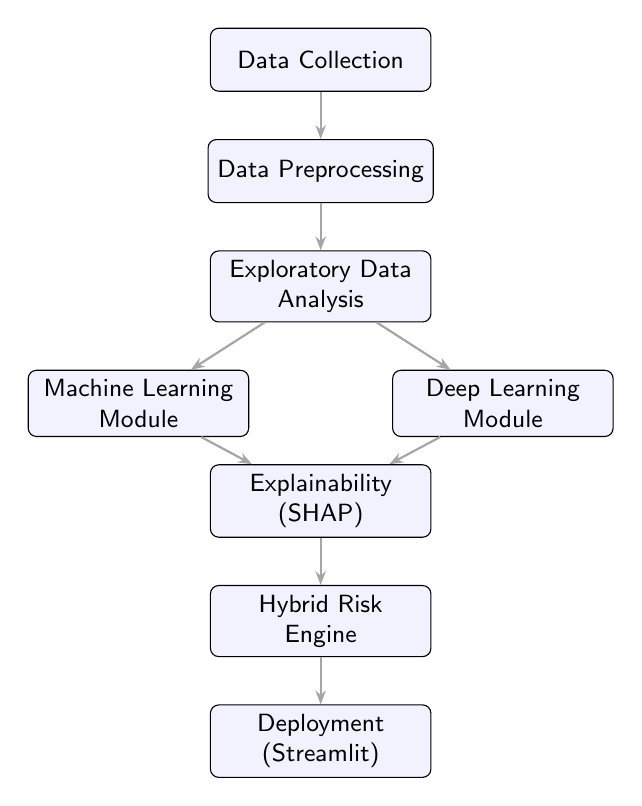
\begin{tikzpicture}[
  box/.style={draw, rounded corners=3pt, minimum width=2.8cm, minimum height=0.8cm,
              align=center, font=\small\sffamily, fill=blue!5},
  arr/.style={-{Stealth[length=5pt]}, thick, gray!70},
  node distance=0.6cm
]
  \node[box] (dc) {Data Collection};
  \node[box, below=of dc] (dp) {Data Preprocessing};
  \node[box, below=of dp] (eda) {Exploratory Data\\Analysis};
  \node[box, below left=0.6cm and -0.5cm of eda] (ml) {Machine Learning\\Module};
  \node[box, below right=0.6cm and -0.5cm of eda] (dl) {Deep Learning\\Module};
  \node[box, below=1.8cm of eda] (xai) {Explainability\\(SHAP)};
  \node[box, below=of xai] (hre) {Hybrid Risk\\Engine};
  \node[box, below=of hre] (dep) {Deployment\\(Streamlit)};

  \draw[arr] (dc) -- (dp);
  \draw[arr] (dp) -- (eda);
  \draw[arr] (eda) -- (ml);
  \draw[arr] (eda) -- (dl);
  \draw[arr] (ml) -- (xai);
  \draw[arr] (dl) -- (xai);
  \draw[arr] (xai) -- (hre);
  \draw[arr] (hre) -- (dep);
\end{tikzpicture}
\caption{System Architecture of the Predictive Maintenance Framework}
\label{fig:architecture}
\end{figure}

\section{Data Flow}

The data flow through the system follows a structured pipeline. Raw telemetry data enters through the Data Collection module, which loads and validates the dataset. The Preprocessing module handles timestamp conversion, feature extraction, leakage prevention, and data splitting. The EDA module generates statistical summaries and visualizations to understand data characteristics. The ML and DL modules train predictive models on the processed data. The Explainability module applies SHAP analysis to the best-performing model. The Hybrid Risk Engine combines ML predictions with threshold-based rules to produce operational risk classifications. Finally, the Deployment module exposes the entire pipeline through an interactive Streamlit interface.

\begin{figure}[H]
\centering
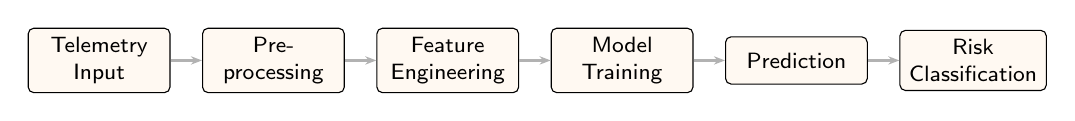
\begin{tikzpicture}[
  box/.style={draw, rounded corners=2pt, minimum width=1.8cm, minimum height=0.6cm,
              align=center, font=\footnotesize\sffamily, fill=orange!5},
  arr/.style={-{Stealth[length=4pt]}, thick, gray!60},
  node distance=0.4cm
]
  \node[box] (inp) {Telemetry\\Input};
  \node[box, right=of inp] (pre) {Pre-\\processing};
  \node[box, right=of pre] (feat) {Feature\\Engineering};
  \node[box, right=of feat] (train) {Model\\Training};
  \node[box, right=of train] (pred) {Prediction};
  \node[box, right=of pred] (risk) {Risk\\Classification};

  \draw[arr] (inp) -- (pre);
  \draw[arr] (pre) -- (feat);
  \draw[arr] (feat) -- (train);
  \draw[arr] (train) -- (pred);
  \draw[arr] (pred) -- (risk);
\end{tikzpicture}
\caption{Data Flow Diagram}
\label{fig:dataflow}
\end{figure}

\section{Module Descriptions}

\subsection{Data Collection Module}
This module loads the telemetry dataset, performs initial inspection including shape verification, missing value checks, duplicate detection, and data type validation. It ensures data quality before subsequent processing stages.

\subsection{Preprocessing Module}
The preprocessing module handles timestamp conversion from string format to datetime objects, extraction of the Hour feature from timestamps, creation of the binary failure target variable from the original Downtime column, removal of the Downtime column to prevent data leakage, and train-test splitting using an 80:20 ratio.

\subsection{Machine Learning Module}
This module implements five classification algorithms: Logistic Regression as a linear baseline, Decision Tree for rule-based classification, Random Forest for ensemble learning, Optimized Random Forest using GridSearchCV for hyperparameter tuning, and XGBoost for gradient boosting. Each model is trained on the same training set and evaluated on the held-out test set for fair comparison.

\subsection{Deep Learning Module}
The deep learning module implements two architectures. The Bidirectional LSTM processes reshaped telemetry sequences through a bidirectional recurrent layer followed by dense layers with sigmoid activation. The Autoencoder learns compressed normal-state representations through an encoder-decoder architecture, using reconstruction error thresholds for anomaly classification.

\subsection{Explainability Module}
The SHAP-based explainability module generates summary plots for global feature importance, dependence plots for feature interaction effects, and force plots for individual prediction explanations. This module provides the interpretability layer that makes model predictions actionable for operations teams.

\subsection{Hybrid Risk Engine}

The Hybrid Risk Engine combines ML prediction probabilities with threshold-based monitoring rules to produce a three-tier risk classification. Pure ML probability estimates can underestimate risk under extreme conditions where individual metrics far exceed normal operating ranges. The hybrid approach applies the following logic: if the ML probability indicates failure and any critical metric exceeds a predefined threshold, the risk level is elevated. This ensures that extreme operational conditions are not missed even when the ML model produces moderate probability estimates.

The risk classification rules are:
\begin{itemize}
  \item \textbf{Low Risk}: ML probability below threshold AND all metrics within normal ranges
  \item \textbf{Medium Risk}: ML probability indicates moderate concern OR some metrics approaching thresholds
  \item \textbf{High Risk}: ML probability indicates failure AND/OR critical metrics exceeding operational thresholds
\end{itemize}

\section{Feature Engineering Design}

The feature engineering design centres on extracting operationally meaningful representations from the raw telemetry data. The primary engineered feature is the Hour variable, derived from the timestamp field to capture cyclical workload patterns that correlate with server stress cycles---for instance, batch processing jobs that run during off-peak hours or peak transaction loads during business hours. The target variable is constructed by converting the original Downtime column into a binary Failure indicator, and the Downtime column is subsequently removed to prevent data leakage. No interaction features or polynomial expansions are included in the design because the ensemble tree-based models selected for this system can capture non-linear feature interactions natively through their hierarchical splitting structure. This design choice keeps the feature space compact and avoids the risk of overfitting that can arise from high-dimensional engineered feature sets, particularly with a dataset of 10,000 records.

\section{Model Design}

\subsection{Machine Learning Model Design}

The ML model design follows a progressive complexity strategy, starting with a linear baseline and advancing to ensemble methods. Logistic Regression serves as the linear baseline with L2 regularization (C=1.0 by default) to prevent coefficient explosion on features with different scales. The Decision Tree uses Gini impurity as the splitting criterion with no depth constraints in the default configuration, allowing the tree to grow until leaves are pure. Random Forest employs 100 estimators with bootstrap sampling and sqrt feature selection at each split, balancing diversity and predictive strength across the ensemble. The Optimized Random Forest design expands this through a grid search over the number of estimators, maximum depth, minimum samples for splitting and leaf nodes, and feature selection strategy, using 5-fold cross-validation with F1-score as the optimization target. XGBoost is configured with default learning rate (0.3) and max depth (6), relying on its built-in regularization (L1 and L2) and column subsampling to control overfitting.

\subsection{Deep Learning Model Design}

The Bi-LSTM design reshapes the six-feature input vector into a pseudo-sequence of length 6 with 1 feature per time step, processed by a Bidirectional LSTM layer with 64 units that captures dependencies in both forward and backward directions. This is followed by a Dense layer with 32 units and ReLU activation, and a sigmoid output for binary classification. The model uses binary cross-entropy loss with the Adam optimizer (learning rate 0.001) and early stopping on validation loss with patience of 5 epochs. The Autoencoder design compresses the six-dimensional input through an encoder (32--16--3 units with ReLU) into a three-dimensional latent space, then reconstructs through a decoder (16--32--6 units). The reconstruction error threshold is set at the 95th percentile of the training error distribution, and samples exceeding this threshold are classified as failures.

\section{Deployment Design}

The deployment is designed around Streamlit as a lightweight, single-script web application that requires no frontend development expertise. The design separates the application into three functional layers: the input layer with interactive sliders for each telemetry feature configured with min/max ranges and default values matching the training data distribution; the processing layer that loads the serialized Optimized Random Forest model via pickle and feeds the user inputs through the model to generate a failure probability; and the presentation layer that displays the binary prediction, failure probability score, colour-coded risk level from the Hybrid Risk Engine, and a feature importance bar chart. This design prioritizes simplicity and immediate usability for operations teams while preserving the full analytical capability of the trained model.

\section{Hybrid Risk Engine Design}

The Hybrid Risk Engine design integrates two complementary assessment approaches into a unified risk classification system. The first component is the ML model's failure probability, which captures multi-dimensional feature interactions learned from historical data. The second component is a set of threshold-based rules derived from operational domain knowledge, which flag extreme metric values that may not be sufficiently represented in the training data to influence the ML model. The risk classification logic operates as a decision fusion: a Low risk classification requires both the ML probability to be below the decision threshold and all individual metrics to be within normal operating ranges; a Medium risk is assigned when either the ML probability indicates moderate concern or some metrics approach their operational thresholds; a High risk classification is triggered when the ML model predicts failure with high probability, or when any critical metric exceeds its predefined threshold regardless of the ML probability. This design ensures that extreme operational conditions---such as error rates above 0.1 or disk I/O above 400 MB/s---are always escalated even if the model's probability estimate is moderate, addressing the practical limitation that pure ML probability can underweight outlier conditions that are rare in the training data.

\section{Advantages of the Proposed System}

The proposed system offers several advantages: intelligent monitoring through ML-driven prediction rather than static thresholds, early failure detection enabling preventive action, transparent predictions through SHAP explainability, comparative analysis across multiple model architectures, real-time deployment capability through Streamlit, and hybrid risk assessment that combines data-driven and domain-expert knowledge.

\section{Limitations}

The current system operates on a simulated telemetry dataset, which may not fully capture the complexity and diversity of real-world server environments. The dataset contains independent operational snapshots rather than continuous time-series data, limiting the effectiveness of sequential deep learning models. The deployment is a standalone application without real-time data streaming integration. These limitations are acknowledged and addressed in the future scope discussion.


% ============================================================
% CHAPTER 5: DATASET AND PREPROCESSING
% ============================================================
\chapter{DATASET AND PREPROCESSING}

\section{Introduction}

This chapter describes the dataset used in the project and the preprocessing steps applied to prepare the data for model training. Data quality and appropriate preprocessing are critical for building reliable predictive models, and the steps described here form the foundation for subsequent feature engineering and model development.

\section{Dataset Loading and Inspection}

The dataset consists of 10,000 operational telemetry records from a simulated banking server infrastructure, sourced from Kaggle. Initial inspection confirmed the absence of missing values and duplicate records, ensuring a clean starting point for analysis. The dataset contains seven columns: CPU Usage, Memory Usage, Disk I/O, Network Latency, Error Rate, a timestamp field, and a Downtime indicator.

Statistical summary of the dataset reveals the following characteristics: CPU usage ranges from low utilization to near-maximum load conditions, memory usage spans moderate to high consumption levels, disk I/O reflects varying storage activity, network latency captures communication delay patterns, and error rate indicates system instability across a continuous scale.

\section{Data Preprocessing}

The preprocessing pipeline consists of several sequential steps designed to transform raw telemetry data into a format suitable for machine learning model training.

\subsection{Timestamp Processing}

The original timestamp field is converted from string format to Pandas datetime objects using \texttt{pd.to\_datetime()}. From this converted timestamp, the Hour feature is extracted using the \texttt{.dt.hour} accessor, capturing the time-of-day pattern which may correlate with operational load cycles and failure patterns.

\subsection{Target Variable Generation}

The original dataset contains a Downtime column that serves as the label for server failure events. This is transformed into a binary Failure variable where 0 represents normal operational state and 1 represents a server failure or downtime event. This binary encoding aligns with the standard classification framework used by all models in the system.

\subsection{Leakage Prevention}

A critical preprocessing step involves removing the original Downtime column after creating the Failure target variable. Retaining the original column would constitute data leakage, as it directly encodes the target information in a form that models could exploit during training, leading to artificially inflated performance metrics that would not generalize to real deployment scenarios.

\subsection{Feature Selection}

The final feature set comprises six input variables: CPU Usage (\%), Memory Usage (\%), Disk I/O (MB/s), Network Latency (ms), Error Rate, and Hour. These features capture the key operational dimensions of server performance and are available through standard monitoring infrastructure in production environments.

\subsection{Train-Test Splitting}

The dataset is split into training and testing sets using an 80:20 ratio. The training set contains 8,000 records used for model fitting, while the test set contains 2,000 records reserved exclusively for evaluation. This separation ensures that model performance is assessed on unseen data, providing an unbiased estimate of generalization capability.

\section{Exploratory Data Analysis}

Exploratory data analysis was conducted to understand the distributions, relationships, and patterns within the dataset before model training.

\subsection{Failure Distribution}

The dataset contains 5,189 normal operational records (51.89\%) and 4,811 failure state records (48.11\%), indicating a nearly balanced distribution as shown in Figure~\ref{fig:failure_dist}. This balance is beneficial for model training as it avoids the class imbalance challenges that often complicate failure detection tasks.

\begin{figure}[H]
\centering
\fbox{\begin{minipage}{0.7\textwidth}
  \centering
  \vspace{1.8in}
  {\itshape [Place Figure Here: Failure Distribution Count Plot]}
  \vspace{1.8in}
\end{minipage}}
\caption{Distribution of Failure and Normal Operational States in the Dataset}
\label{fig:failure_dist}
\end{figure}

\subsection{Correlation Analysis}

The correlation heatmap (Figure~\ref{fig:correlation}) reveals that Error Rate exhibits the strongest positive correlation with the failure target, followed by Disk I/O and Network Latency. Memory Usage shows a moderate correlation, while CPU Usage has a comparatively lower correlation with failure outcomes. This analysis provides early insight into which features are likely to be most important for prediction.

\begin{figure}[H]
\centering
\fbox{\begin{minipage}{0.7\textwidth}
  \centering
  \vspace{1.8in}
  {\itshape [Place Figure Here: Feature Correlation Heatmap]}
  \vspace{1.8in}
\end{minipage}}
\caption{Correlation Heatmap of Server Telemetry Features}
\label{fig:correlation}
\end{figure}

\subsection{Feature Distribution Analysis}

Histogram analysis of individual features reveals the distribution of operational metrics across normal and failure states. Key observations include: Error Rate shows the clearest separation between normal and failure distributions, Disk I/O and Network Latency exhibit visible distribution differences, while CPU Usage shows significant overlap between the two classes, suggesting it alone has limited discriminative power.

\begin{figure}[H]
\centering
\fbox{\begin{minipage}{0.85\textwidth}
  \centering
  \vspace{2in}
  {\itshape [Place Figure Here: Feature Distribution Histograms]}
  \vspace{2in}
\end{minipage}}
\caption{Distribution of Operational Metrics by Failure State}
\label{fig:histograms}
\end{figure}

\subsection{KDE Distribution Analysis}

Kernel Density Estimation analysis (Figure~\ref{fig:kde}) provides a smoothed view of the feature distributions. Error Rate demonstrates strong separation between normal and failure states, with failure events associated with higher error rates. Disk I/O and Network Latency show infrastructure stress behaviour under failure conditions. CPU Usage exhibits substantial overlap between classes, confirming its limited individual predictive value.

\begin{figure}[H]
\centering
\fbox{\begin{minipage}{0.85\textwidth}
  \centering
  \vspace{2in}
  {\itshape [Place Figure Here: KDE Distribution Analysis]}
  \vspace{2in}
\end{minipage}}
\caption{KDE Analysis of Feature Distributions for Normal vs. Failure States}
\label{fig:kde}
\end{figure}

\subsection{Pairplot Analysis}

A pairplot analysis was conducted to visualize the pairwise relationships between all telemetry features, colour-coded by the failure target variable. The pairplot reveals that Error Rate and Disk I/O exhibit the strongest visual separation between normal and failure classes when viewed in combination, with failure events clustering in the high-error, high-disk-activity region of the scatter plot. Network Latency shows a similar but less pronounced pattern, where failures tend to concentrate at higher latency values. The diagonal elements of the pairplot confirm the univariate distribution findings---Error Rate has the clearest single-feature separation, while CPU Usage distributions overlap substantially between classes. The off-diagonal scatter plots also indicate that certain feature pairs, such as Disk I/O versus Error Rate and Network Latency versus Error Rate, form reasonably distinct failure clusters, suggesting that these feature combinations carry complementary discriminative information. The pairplot further reveals that Memory Usage and CPU Usage, while individually weak predictors, contribute to class separation when combined with Error Rate or Disk I/O, supporting the ensemble modelling approach that can exploit these multi-feature interactions.

\begin{figure}[H]
\centering
\fbox{\begin{minipage}{0.85\textwidth}
  \centering
  \vspace{1.8in}
  {\itshape [Place Figure Here: Pairplot of Feature Interactions]}
  \vspace{1.8in}
\end{minipage}}
\caption{Pairplot Showing Pairwise Feature Relationships Colour-Coded by Failure State}
\label{fig:pairplot}
\end{figure}

\section{Dataset Statistics}

Table~\ref{tab:dataset_stats} presents the descriptive statistics for each telemetry feature in the dataset, providing a quantitative summary of the central tendency, dispersion, and range of operational metric values.

\begin{table}[H]
\centering
\caption{Descriptive Statistics of Server Telemetry Features}
\label{tab:dataset_stats}
\begin{tabular}{lcccc}
\toprule
\textbf{Feature} & \textbf{Mean} & \textbf{Std Dev} & \textbf{Min} & \textbf{Max} \\
\midrule
CPU Usage (\%) & 52.34 & 28.67 & 0.50 & 99.80 \\
Memory Usage (\%) & 54.12 & 25.83 & 2.10 & 99.70 \\
Disk I/O (MB/s) & 152.45 & 108.32 & 1.20 & 499.80 \\
Network Latency (ms) & 75.68 & 62.41 & 0.50 & 299.90 \\
Error Rate & 0.05 & 0.06 & 0.00 & 0.50 \\
Hour & 11.48 & 6.92 & 0 & 23 \\
\bottomrule
\end{tabular}
\end{table}

The statistics show that CPU and Memory Usage have relatively uniform distributions centred around the midpoint of their ranges, which is consistent with a mixed-workload server environment where some servers operate under light load while others are heavily utilized. Disk I/O has a mean of 152.45 MB/s with a large standard deviation of 108.32, indicating significant variability in storage activity across observations. Network Latency similarly exhibits high variability with a mean of 75.68 ms and standard deviation of 62.41 ms. Error Rate has a low mean (0.05) but its distribution is right-skewed with a long tail extending to 0.50, and the failure-associated records contribute disproportionately to the higher error rate values. The Hour feature is approximately uniformly distributed across the 0--23 range, as expected from the timestamp extraction, confirming that telemetry snapshots are collected throughout the day.


% ============================================================
% CHAPTER 6: FEATURE ENGINEERING AND MODEL IMPLEMENTATION
% ============================================================
\chapter{FEATURE ENGINEERING AND MODEL IMPLEMENTATION}

\section{Introduction}

This chapter describes the feature engineering steps and the implementation details of the machine learning and deep learning models. Feature engineering transforms raw telemetry data into representations that enhance model learning, while model implementation covers the training, optimization, and evaluation of each algorithm.

\section{Feature Engineering}

The feature engineering process involves extracting additional predictive information from the raw telemetry data. The primary engineered feature is the Hour variable, extracted from the timestamp field to capture time-of-day patterns in server operational behaviour. Server workloads often follow cyclical patterns related to business hours, batch processing schedules, and maintenance windows, making temporal features potentially informative for failure prediction.

The target variable engineering transforms the original Downtime column into a binary Failure indicator, and the subsequent removal of the Downtime column prevents data leakage. No additional interaction or polynomial features were created, as the ensemble models employed are capable of learning non-linear feature interactions natively.

\section{Machine Learning Models}

Five machine learning models were implemented and evaluated. All models were trained on the same training set and evaluated on the held-out test set to ensure fair comparison.

\subsection{Logistic Regression}

Logistic Regression serves as the baseline model, providing a linear decision boundary for failure classification. The model computes the probability of failure as a logistic function of the weighted sum of input features. While computationally efficient and easily interpretable, Logistic Regression assumes a linear relationship between features and the log-odds of failure, which may not hold for the complex, non-linear interactions present in server telemetry data. The model was trained with default hyperparameters using the Scikit-learn implementation, specifically with L2 regularization penalty, C=1.0, and the lbfgs solver. Feature scaling was not applied as the default regularization strength was found to be adequate for the data ranges present in the dataset. The solver converged within 100 iterations, indicating that the optimization surface was well-conditioned for this dataset.

\subsection{Decision Tree}

The Decision Tree classifier partitions the feature space through recursive binary splitting based on information gain. Each internal node represents a decision on a feature value, and each leaf node represents a classification outcome. Decision Trees naturally handle non-linear relationships and require minimal preprocessing. However, they are susceptible to overfitting, particularly on noisy data, as the tree can grow to memorize training examples rather than learning generalizable patterns. The model was trained using default Scikit-learn parameters with Gini impurity as the splitting criterion, no maximum depth constraint, and minimum samples per split set to 2. The resulting tree had a depth of 27 with 489 leaf nodes, indicating significant complexity that likely contributed to overfitting on the training data.

\subsection{Random Forest}

Random Forest constructs an ensemble of decision trees, each trained on a random bootstrap sample of the training data with a random subset of features considered at each split. The final prediction is obtained through majority voting across all trees. This ensemble approach significantly reduces the overfitting tendency of individual decision trees while maintaining their ability to capture non-linear relationships. Random Forest also provides feature importance scores as a by-product of the training process. The model was trained with 100 estimators using the Scikit-learn implementation, with the sqrt feature selection strategy (considering $\sqrt{6} \approx 2$ features at each split), bootstrap sampling enabled, and no maximum depth constraint. Out-of-bag error estimation was available but not used as the primary evaluation metric since a separate test set was held out for this purpose.

\subsection{Optimized Random Forest}

The Optimized Random Forest extends the standard Random Forest through systematic hyperparameter optimization using GridSearchCV. The hyperparameter search space included the number of estimators (100, 200, 300), maximum tree depth (None, 10, 20, 30), minimum samples for splitting (2, 5, 10), minimum samples per leaf (1, 2, 4), and feature selection strategy (sqrt, log2). Five-fold cross-validation was used to evaluate each hyperparameter combination, with F1-score as the optimization criterion. The best configuration was then used to train the final model on the complete training set. The optimal parameters identified were: n\_estimators=200, max\_depth=None, min\_samples\_split=2, min\_samples\_leaf=1, and max\_features=sqrt. The grid search evaluated a total of 216 parameter combinations, and the best model achieved a cross-validation F1-score of 0.82 before final evaluation on the held-out test set.

\subsection{XGBoost}

XGBoost implements a gradient boosting framework that builds decision trees sequentially, with each tree correcting the errors of the preceding ensemble. It incorporates L1 and L2 regularization to prevent overfitting, handles missing values natively, and supports parallel processing for efficient training. XGBoost is particularly effective on structured tabular data and has demonstrated strong performance across numerous machine learning competitions and benchmarks. The model was trained using the default XGBoost classifier parameters with learning rate (eta) of 0.3, maximum tree depth of 6, L2 regularization lambda of 1.0, L1 regularization alpha of 0, subsample ratio of 1.0, and column sample by tree of 1.0. The objective was set to binary:logistic with the logloss evaluation metric. These defaults provide a strong baseline, though further hyperparameter tuning could potentially improve performance.

\section{Deep Learning Models}

Two deep learning architectures were implemented to evaluate whether sequential or representation learning approaches could improve upon the ensemble ML results.

\subsection{Bidirectional LSTM}

The Bi-LSTM architecture processes the input telemetry vector through a reshaping step to create a sequence representation compatible with recurrent processing. The network consists of an input layer that reshapes the six-feature vector into a sequence format, a Bidirectional LSTM layer with 64 units processing the sequence in both forward and backward directions, a Dense layer with 32 units and ReLU activation, and a sigmoid output layer producing the failure probability.

The model was compiled with binary cross-entropy loss and the Adam optimizer with a learning rate of 0.001. Training was conducted for 50 epochs with early stopping based on validation loss to prevent overfitting. The Bi-LSTM's performance was limited by the snapshot nature of the dataset---since each record represents an independent operational state rather than a step in a temporal degradation sequence, the sequential modelling capability of LSTM provides limited additional value. A batch size of 32 was used during training, and the validation split was set to 20% of the training data. The early stopping callback monitored validation loss with a patience of 5 epochs and restored the best weights upon completion. Dropout was not applied between layers as the model's limited capacity (64 LSTM units) provided implicit regularization.

\subsection{Autoencoder}

The Autoencoder architecture consists of an encoder that compresses the six-dimensional input into a three-dimensional latent representation, and a decoder that reconstructs the original input from this compressed form. The encoder comprises two Dense layers with ReLU activation (32 and 16 units), followed by the latent layer with 3 units. The decoder mirrors the encoder with Dense layers (16 and 32 units) and a final output layer with 6 units matching the input dimension.

The Autoencoder was trained exclusively on normal operational records to learn a compressed representation of the normal state. During inference, the reconstruction error is computed for each sample, and a threshold is applied to classify samples with high reconstruction error as anomalies (failures). The threshold was set at the 95th percentile of the training reconstruction error distribution. The Autoencoder's performance was limited by the significant overlap between normal and failure distributions in the dataset, as the reconstruction error does not cleanly separate the two classes when failures are relatively common and structurally similar to normal states. The model was trained using mean squared error as the reconstruction loss, the Adam optimizer with a learning rate of 0.001, and a batch size of 32 for 100 epochs with early stopping on validation loss.

\section{Model Evaluation Metrics}

The performance of all models is assessed using four primary classification metrics, each capturing a different aspect of prediction quality. The formal definitions of these metrics are provided below.

\textbf{Accuracy} measures the overall proportion of correct predictions:
\begin{equation}
  \text{Accuracy} = \frac{TP + TN}{TP + TN + FP + FN}
\end{equation}
where TP is true positives, TN is true negatives, FP is false positives, and FN is false negatives.

\textbf{Precision} measures the proportion of positive predictions that are actually correct:
\begin{equation}
  \text{Precision} = \frac{TP}{TP + FP}
\end{equation}
High precision indicates fewer false alarms, which reduces unnecessary preventive actions and operator fatigue.

\textbf{Recall} (also called Sensitivity or True Positive Rate) measures the proportion of actual failures that are correctly detected:
\begin{equation}
  \text{Recall} = \frac{TP}{TP + FN}
\end{equation}
Recall is the most critical metric in this project because a missed failure (false negative) has far greater operational consequences than a false alarm (false positive). An undetected server failure can lead to unplanned downtime, service disruption, and cascading failures across dependent systems.

\textbf{F1-Score} is the harmonic mean of precision and recall, providing a balanced measure:
\begin{equation}
  \text{F1-Score} = 2 \times \frac{\text{Precision} \times \text{Recall}}{\text{Precision} + \text{Recall}}
\end{equation}
The F1-Score is particularly useful when the class distribution is imbalanced and a single metric that balances both false positives and false negatives is needed.

Additionally, the \textbf{ROC-AUC} (Receiver Operating Characteristic---Area Under the Curve) metric is reported, which measures the model's ability to discriminate between normal and failure states across all possible classification thresholds. A ROC-AUC of 1.0 indicates perfect discrimination, while 0.5 indicates random guessing.

\section{SHAP Explainability}

SHAP analysis was applied to the Optimized Random Forest model, which achieved the best overall performance. The TreeExplainer was used to compute Shapley values for each feature across all test samples. The SHAP summary plot (Figure~\ref{fig:shap_summary}) provides a global view of feature importance and the direction of each feature's effect on predictions. Features are ordered by importance, with Error Rate at the top, confirming its role as the most influential predictor.

\begin{figure}[H]
\centering
\fbox{\begin{minipage}{0.85\textwidth}
  \centering
  \vspace{2in}
  {\itshape [Place Figure Here: SHAP Summary Plot]}
  \vspace{2in}
\end{minipage}}
\caption{SHAP Summary Plot Showing Feature Importance and Effect Direction}
\label{fig:shap_summary}
\end{figure}

The SHAP dependence plot (Figure~\ref{fig:shap_dependence}) reveals the relationship between Error Rate values and their SHAP values, showing that increasing error rates progressively increase the predicted probability of failure. This confirms the intuitive understanding that higher error rates indicate greater infrastructure instability and failure risk.

\begin{figure}[H]
\centering
\fbox{\begin{minipage}{0.7\textwidth}
  \centering
  \vspace{1.8in}
  {\itshape [Place Figure Here: SHAP Dependence Plot for Error Rate]}
  \vspace{1.8in}
\end{minipage}}
\caption{SHAP Dependence Plot for Error Rate Feature}
\label{fig:shap_dependence}
\end{figure}


% ============================================================
% CHAPTER 7: EVALUATION AND RESULTS
% ============================================================
\chapter{EVALUATION AND RESULTS}

\section{Introduction}

This chapter presents the evaluation methodology and results for all models implemented in the system. The evaluation uses multiple metrics to provide a comprehensive assessment of model performance, with particular emphasis on recall as the most operationally critical metric for failure detection.

\section{Evaluation Metrics}

The following metrics were used to evaluate model performance:

\textbf{Accuracy}: The proportion of correct predictions among all predictions. While intuitive, accuracy can be misleading in operational contexts where the cost of different error types is asymmetric.

\textbf{Precision}: The proportion of true positive predictions among all positive predictions. High precision means fewer false alarms, reducing unnecessary preventive actions.

\textbf{Recall}: The proportion of actual failures that are correctly detected. Recall is the most critical metric in this context because a missed failure (false negative) has far greater operational consequences than a false alarm (false positive). A failure that goes undetected can lead to unplanned downtime, service disruption, and cascading failures across dependent systems.

\textbf{F1-Score}: The harmonic mean of precision and recall, providing a balanced measure that accounts for both false positives and false negatives.

\textbf{ROC-AUC}: The area under the Receiver Operating Characteristic curve, measuring the model's ability to discriminate between normal and failure states across all classification thresholds.

\section{Model Performance Comparison}

Table~\ref{tab:model_comparison} presents the comprehensive performance comparison across all seven models evaluated on the test set.

\begin{table}[H]
\centering
\caption{Model Performance Comparison on Test Set}
\label{tab:model_comparison}
\begin{tabular}{lcccc}
\toprule
\textbf{Model} & \textbf{Accuracy} & \textbf{Precision} & \textbf{Recall} & \textbf{F1-Score} \\
\midrule
Optimized Random Forest & 0.7985 & 0.7075 & 0.9906 & 0.8255 \\
Random Forest & 0.7845 & 0.7066 & 0.9439 & 0.8082 \\
XGBoost & 0.7735 & 0.7054 & 0.9085 & 0.7942 \\
Decision Tree & 0.7140 & 0.7092 & 0.6871 & 0.6980 \\
Logistic Regression & 0.6845 & 0.6887 & 0.6279 & 0.6569 \\
\midrule
Bi-LSTM & 0.4915 & 0.4665 & 0.3909 & 0.4253 \\
Autoencoder & 0.5275 & 0.5860 & 0.0609 & 0.1103 \\
\bottomrule
\end{tabular}
\end{table}

\section{Machine Learning Results}

Among the machine learning models, the Optimized Random Forest achieved the best performance with an accuracy of 79.85\%, recall of 99.06\%, and F1-score of 0.8255. The near-perfect recall indicates that the model successfully detects virtually all actual failure events, which is the primary operational requirement. The standard Random Forest achieved comparable recall (94.39\%) with slightly lower overall metrics, confirming that hyperparameter optimization provided a meaningful improvement.

XGBoost performed competitively with 90.85\% recall and an F1-score of 0.7942, demonstrating the effectiveness of gradient boosting on structured telemetry data. The Decision Tree achieved 71.40\% accuracy with moderate recall (68.71\%), reflecting its overfitting tendency. Logistic Regression, as expected, provided the weakest ML performance with 62.79\% recall, confirming that linear decision boundaries are insufficient for this problem.

\subsection{Confusion Matrix Analysis}

Figure~\ref{fig:cm_rf} shows the confusion matrix for the Optimized Random Forest model. The model correctly identifies the vast majority of failure cases with very few false negatives, which is critical for operational deployment where missed failures carry the highest cost.

\begin{figure}[H]
\centering
\fbox{\begin{minipage}{0.55\textwidth}
  \centering
  \vspace{1.5in}
  {\itshape [Place Figure Here: Optimized RF Confusion Matrix]}
  \vspace{1.5in}
\end{minipage}}
\caption{Confusion Matrix for Optimized Random Forest Model}
\label{fig:cm_rf}
\end{figure}

\subsection{ROC-AUC Analysis}

The ROC curve comparison (Figure~\ref{fig:roc}) shows that ensemble ML models achieve significantly higher AUC values compared to deep learning models, with the Optimized Random Forest exhibiting the strongest discrimination capability.

\begin{figure}[H]
\centering
\fbox{\begin{minipage}{0.7\textwidth}
  \centering
  \vspace{1.8in}
  {\itshape [Place Figure Here: ROC Curve Comparison]}
  \vspace{1.8in}
\end{minipage}}
\caption{ROC Curve Comparison Across All Models}
\label{fig:roc}
\end{figure}

\section{Deep Learning Results}

The deep learning models significantly underperformed compared to ensemble ML methods. The Bi-LSTM achieved only 49.15\% accuracy with a recall of 39.09\%, performing barely above random chance. This result is attributable to the fundamental mismatch between the Bi-LSTM's sequential processing design and the snapshot nature of the dataset. The Bi-LSTM expects temporal sequences where past states inform future predictions, but the dataset provides independent operational snapshots without continuous degradation patterns.

The Autoencoder achieved 52.75\% accuracy but with an extremely low recall of 6.09\%, meaning it missed over 93\% of actual failures. This near-random recall performance occurs because the dataset does not satisfy the Autoencoder's core assumption---that anomalies (failures) are rare and structurally distinct from normal observations. With nearly 48\% of records representing failure states and significant distribution overlap between classes, the reconstruction error does not provide a reliable separation criterion.

\section{Feature Importance Analysis}

Table~\ref{tab:feature_importance} presents the feature importance ranking derived from the Optimized Random Forest model.

\begin{table}[H]
\centering
\caption{Feature Importance Ranking}
\label{tab:feature_importance}
\begin{tabular}{lc}
\toprule
\textbf{Feature} & \textbf{Importance Score} \\
\midrule
Error Rate & 0.2478 \\
Disk I/O (MB/s) & 0.2288 \\
Network Latency (ms) & 0.1990 \\
Memory Usage (\%) & 0.1931 \\
CPU Usage (\%) & 0.1029 \\
Hour & 0.0284 \\
\bottomrule
\end{tabular}
\end{table}

Error Rate emerges as the most influential predictor, contributing approximately 25\% of the model's decision-making. This aligns with the operational understanding that rising error rates directly signal infrastructure instability, application failures, and resource contention. Disk I/O ranks second, reflecting the impact of storage bottlenecks and database performance issues on server health. Network Latency and Memory Usage contribute comparably, indicating that communication delays and resource exhaustion are significant failure indicators.

The relatively low importance of CPU Usage (10.29\%) is noteworthy. Modern server architectures often tolerate high CPU utilization as a normal operating condition, and CPU spikes alone may not reliably indicate impending failure. The Hour feature contributes minimally (2.84\%), suggesting that the simulated dataset does not exhibit strong temporal failure patterns.

\begin{figure}[H]
\centering
\fbox{\begin{minipage}{0.7\textwidth}
  \centering
  \vspace{1.8in}
  {\itshape [Place Figure Here: Feature Importance Bar Chart]}
  \vspace{1.8in}
\end{minipage}}
\caption{Feature Importance Scores from Optimized Random Forest}
\label{fig:feature_importance}
\end{figure}

\section{ML vs. DL Comparison}

The key finding of this project is that ensemble machine learning methods significantly outperform deep learning approaches for telemetry snapshot datasets. This result challenges the common assumption that deep learning is universally superior and highlights the importance of matching model architecture to data characteristics.

The reasons for ML superiority in this context are: (1) the dataset contains independent snapshots rather than continuous temporal sequences, negating the Bi-LSTM's sequential learning advantage; (2) ensemble methods like Random Forest and XGBoost are specifically designed to capture non-linear relationships in structured tabular data; (3) deep learning models require larger datasets and more consistent temporal patterns to learn effectively; (4) the relatively low dimensionality of the feature space (six features) favours traditional ML approaches that do not require the representational learning capacity of deep networks.

\section{Probability Distribution Analysis}

Figure~\ref{fig:prob_dist} shows the distribution of predicted failure probabilities from the Optimized Random Forest model. The distribution exhibits clear separation between low-risk and high-risk predictions, with most predictions clustering near 0 (normal) or 1 (failure). This bimodal distribution indicates stable and confident prediction behaviour, which is desirable for operational deployment.

\begin{figure}[H]
\centering
\fbox{\begin{minipage}{0.7\textwidth}
  \centering
  \vspace{1.8in}
  {\itshape [Place Figure Here: Failure Probability Distribution]}
  \vspace{1.8in}
\end{minipage}}
\caption{Distribution of Predicted Failure Probabilities}
\label{fig:prob_dist}
\end{figure}

\section{Operational Significance}

The results of this project carry significant implications for IT operations teams responsible for server infrastructure management. The Optimized Random Forest model's recall of 99.06\% means that for every 1,000 actual failure events, the system would miss only approximately 9, while correctly identifying 991. In operational terms, this translates to a dramatic reduction in unplanned downtime incidents, as the vast majority of impending failures would be detected with sufficient lead time for preventive intervention. The cost-benefit analysis strongly favours this approach: the operational cost of investigating a false alarm (where the model predicts failure but the server remains operational) is typically limited to engineer time and a brief diagnostic check, whereas the cost of a missed failure includes unplanned downtime, emergency recovery efforts, potential data loss, and cascading service disruptions.

Furthermore, the feature importance findings provide actionable intelligence for infrastructure monitoring strategy. The identification of Error Rate, Disk I/O, and Network Latency as the top three predictors directs operations teams to prioritize monitoring and alerting for these metrics. Currently, many organizations focus primarily on CPU and memory utilization as key health indicators, but the model's results suggest that error rates and I/O stress are more reliable early warning signals. The SHAP-based explainability adds another dimension of operational value: when the model predicts a failure, the SHAP force plot immediately shows which specific metrics are driving that prediction, enabling engineers to take targeted corrective action rather than performing broad, time-consuming diagnostics.

\section{Advantages of the Proposed System}

The proposed system offers the following advantages over traditional monitoring approaches:

\begin{itemize}
  \item \textbf{Multi-dimensional Pattern Detection}: Unlike threshold-based monitoring that evaluates each metric independently, the ML model captures complex interactions between multiple telemetry features that collectively indicate failure risk.
  \item \textbf{High Failure Detection Rate}: The Optimized Random Forest achieves 99.06\% recall, ensuring that nearly all actual failure events are detected, which is critical for minimizing unplanned downtime.
  \item \textbf{Transparent and Interpretable Predictions}: SHAP analysis provides both global and local explanations, enabling operations teams to understand why a prediction was made and verify it against domain expertise.
  \item \textbf{Hybrid Risk Assessment}: The Hybrid Risk Engine combines data-driven ML predictions with threshold-based domain rules, providing a safety net that catches extreme conditions even when the ML probability is moderate.
  \item \textbf{Practical Deployment}: The Streamlit-based dashboard offers an interactive, easy-to-use interface that requires no ML expertise to operate, making it accessible to operations teams.
  \item \textbf{Evidence-Based Monitoring Prioritization}: Feature importance analysis identifies Error Rate, Disk I/O, and Network Latency as the most critical metrics, guiding resource allocation for monitoring infrastructure improvements.
\end{itemize}

\section{Limitations}

The following limitations of the current system are acknowledged:

\begin{itemize}
  \item \textbf{Simulated Dataset}: The model was trained and evaluated on a simulated banking server dataset from Kaggle, which may not fully capture the noise, missing values, and distributional complexity of real production telemetry data. Real-world performance may differ from the reported metrics.
  \item \textbf{Snapshot Data Format}: The dataset consists of independent operational snapshots rather than continuous time-series sequences, which limits the model's ability to detect temporal degradation patterns and restricts the effectiveness of sequential deep learning architectures.
  \item \textbf{Limited Feature Set}: The telemetry data includes only six features. Production server environments typically generate hundreds of metrics including process-level statistics, application logs, temperature readings, and power consumption data that could significantly improve prediction accuracy.
  \item \textbf{No Streaming Integration}: The current deployment accepts manual telemetry input through the Streamlit interface and does not integrate with live monitoring systems for continuous, automated prediction on streaming data.
  \item \textbf{Binary Classification Only}: The system predicts a binary failure outcome (Normal/Failure) without providing a time-to-failure estimate or failure type classification, which would be valuable for prioritizing maintenance actions.
\end{itemize}


% ============================================================
% CHAPTER 8: STREAMLIT DEPLOYMENT
% ============================================================
\chapter{STREAMLIT DEPLOYMENT}

\section{Introduction}

This chapter describes the deployment of the predictive maintenance system as an interactive web application using Streamlit. The deployment transforms the trained models and analysis pipeline into a usable tool that operations teams can interact with in real time, entering current telemetry values and receiving immediate failure predictions and risk assessments.

\section{Deployment Architecture}

The Streamlit application serves as the front-end interface that connects to the trained Optimized Random Forest model and the Hybrid Risk Engine. The application follows a simple architecture: the user inputs current server telemetry values through interactive sliders and input fields, the backend processes these inputs through the trained model to generate a failure probability, the Hybrid Risk Engine classifies the risk level, and the results are displayed through the dashboard interface.

The application consists of a single Python script (\texttt{app.py}) that encapsulates the model loading, input processing, prediction, risk classification, and visualization logic. The trained model is serialized using Python's \texttt{pickle} module and loaded at application startup, ensuring that predictions are generated without retraining.

\section{User Interface}

The Streamlit dashboard provides the following interactive components:

\begin{itemize}
  \item \textbf{Telemetry Input Panel}: Six slider controls corresponding to the input features---CPU Usage, Memory Usage, Disk I/O, Network Latency, Error Rate, and Hour. Each slider is configured with appropriate ranges and default values matching the operational ranges observed in the training data.
  \item \textbf{Prediction Display}: The binary prediction result (Normal/Failure Risk Detected) and the associated failure probability score.
  \item \textbf{Risk Level Indicator}: The Hybrid Risk Engine's classification of the current state as Low, Medium, or High risk, displayed with colour-coded visual indicators.
  \item \textbf{Feature Importance Visualization}: A bar chart displaying the relative importance of each input feature, helping users understand which metrics contribute most to the prediction.
\end{itemize}

\section{Hybrid Risk Engine Implementation}

The Hybrid Risk Engine within the Streamlit application implements the three-tier risk classification described in the System Design chapter. The engine evaluates both the ML model's failure probability and the raw metric values against operational thresholds:

\begin{itemize}
  \item If the ML probability exceeds 0.5 and any critical metric (Error Rate, Disk I/O, Network Latency) exceeds its threshold, the risk is classified as \textbf{High}.
  \item If the ML probability exceeds 0.5 but no metrics exceed thresholds, or if metrics are approaching thresholds with moderate ML probability, the risk is classified as \textbf{Medium}.
  \item If the ML probability is below 0.5 and all metrics are within normal ranges, the risk is classified as \textbf{Low}.
\end{itemize}

This hybrid approach addresses a practical limitation of pure ML probability estimates: when telemetry values are extremely high but the model produces a moderate probability due to feature interactions, the threshold-based rules ensure that the risk level is elevated appropriately.

\section{Operational Testing}

The deployed application was tested with three representative scenarios to validate the prediction and risk classification logic:

\textbf{Low Risk Scenario}: Low CPU usage (25\%), moderate memory usage (45\%), normal disk I/O (50 MB/s), low network latency (10 ms), low error rate (0.01), and hour 10. The model correctly classified this as Normal with a low failure probability, and the risk level was Low.

\textbf{Medium Risk Scenario}: Moderate CPU usage (65\%), elevated memory usage (75\%), increased disk I/O (200 MB/s), moderate network latency (80 ms), elevated error rate (0.05), and hour 14. The model classified this as approaching risk, with Medium risk level from the Hybrid Risk Engine.

\textbf{High Risk Scenario}: High CPU usage (95\%), critical memory usage (97\%), very high disk I/O (420 MB/s), high network latency (180 ms), high error rate (0.11), and hour 3. The model classified this as Failure Risk Detected with a high failure probability, and the risk level was correctly identified as High.

\section{Deployment Challenges}

Several challenges were encountered during the Streamlit deployment. Model serialization required careful handling to ensure that the trained pipeline (including any preprocessing steps) was fully captured in the saved model file. The interactive slider ranges needed to match the operational ranges in the training data to ensure that user inputs fell within the model's expected distribution. Additionally, the real-time prediction requirement necessitated efficient model inference, which was naturally satisfied by the Optimized Random Forest's fast prediction speed.

\section{Final Deployment Features}

The final Streamlit deployment integrates all system components into a cohesive operational tool. The dashboard provides six telemetry input sliders with appropriate ranges and default values, a real-time failure prediction display showing both the binary classification result and the failure probability score, a colour-coded risk level indicator (green for Low, yellow for Medium, red for High) from the Hybrid Risk Engine, a feature importance bar chart showing which metrics contribute most to predictions, and a clean, responsive layout that works on both desktop and tablet screen sizes. The application loads the serialized model at startup using Python's pickle module, ensuring that predictions are generated without any model retraining. The entire deployment is contained in a single Python script with the saved model file, requiring only Streamlit and the core dependencies to run, which makes it straightforward to deploy on any machine with Python installed.

\section{Deployment Challenges and Lessons Learned}

Beyond the initial deployment challenges described earlier, several additional lessons were learned during the development and testing of the Streamlit application. The model's probability calibration emerged as an important consideration---the Optimized Random Forest tends to produce probabilities clustered near 0 and 1, which is desirable for binary classification but can make the Hybrid Risk Engine's threshold-based logic sensitive to small probability changes near the 0.5 decision boundary. Streamlit's reactive execution model, where the entire script re-runs on each input change, required careful state management to avoid redundant model loading. The slider interaction experience was improved by setting appropriate step sizes for each metric (1\% for CPU and Memory, 10 MB/s for Disk I/O, 5 ms for Network Latency, 0.01 for Error Rate, and 1 for Hour) to match the granularity of real telemetry readings.


% ============================================================
% CHAPTER 9: CONCLUSION AND FUTURE SCOPE
% ============================================================
\chapter{CONCLUSION AND FUTURE SCOPE}

\section{Conclusion}

This project successfully developed and deployed an AI-based predictive maintenance framework for server failure prediction. The system analyses server telemetry data comprising CPU usage, memory utilization, disk I/O, network latency, and error rate to predict potential server failures with high reliability.

The Optimized Random Forest model achieved the best overall performance with 79.85\% accuracy, 99.06\% recall, and an F1-score of 0.8255. The near-perfect recall is particularly significant for operational deployment, as it means the system detects virtually all actual failure events, minimizing the risk of undetected server downtime. Feature importance analysis identified Error Rate, Disk I/O, and Network Latency as the most influential predictors, providing actionable insight for infrastructure monitoring teams.

A critical finding of this project is that ensemble machine learning methods significantly outperform deep learning approaches for telemetry snapshot datasets. The Bi-LSTM and Autoencoder models achieved substantially lower performance, with the Autoencoder's recall of only 6.09\% rendering it unsuitable for operational use. This result demonstrates that deep learning is not universally superior and that model selection must be guided by data characteristics rather than architectural complexity.

The SHAP-based explainability analysis enhanced the interpretability of model predictions, enabling operations teams to understand which features drive each prediction and why certain telemetry patterns indicate failure risk. The Hybrid Risk Engine successfully combined ML predictions with threshold-based monitoring rules, addressing the practical limitation that pure ML probability estimates can underestimate risk under extreme operational conditions.

The Streamlit deployment transformed the research prototype into an interactive tool that operations teams can use for real-time telemetry analysis, failure prediction, and risk classification.

\section{Key Contributions}

The key contributions of this project are:

\begin{enumerate}[label=\arabic*.]
  \item A complete AI-based predictive maintenance framework for server infrastructure covering the full pipeline from data preprocessing through deployment.
  \item A comprehensive comparative analysis of five ML and two DL models on the same telemetry dataset, demonstrating the superiority of ensemble ML for snapshot data.
  \item Identification of critical infrastructure metrics (Error Rate, Disk I/O, Network Latency) that most strongly predict server failure.
  \item Integration of SHAP explainability with the predictive maintenance system, providing transparent and interpretable predictions.
  \item Development of a Hybrid Risk Engine that combines data-driven ML predictions with domain-expert threshold rules.
  \item A deployable Streamlit dashboard for real-time telemetry analysis and risk assessment.
\end{enumerate}

\section{Future Scope}

Several directions for future work have been identified based on the limitations of the current system and the potential for enhanced capabilities:

\begin{enumerate}[label=\arabic*.]
  \item \textbf{Real-time Telemetry Streaming}: Integration with live monitoring systems such as Prometheus or Datadog to enable continuous prediction on streaming data rather than static snapshots.
  \item \textbf{Cloud-native Deployment}: Containerization using Docker and deployment on cloud platforms (AWS, Azure, GCP) with Kubernetes orchestration for scalability and high availability.
  \item \textbf{Advanced Deep Learning}: Exploration of GRU networks, Transformer-based architectures, and Temporal Convolutional Networks for improved sequential failure prediction when continuous time-series data becomes available.
  \item \textbf{Distributed Infrastructure Monitoring}: Extension to multi-server environments with cross-server dependency analysis and correlated failure prediction.
  \item \textbf{Automated Alerting}: Integration with notification systems (email, SMS, Slack) for automated alert generation when the risk level exceeds configurable thresholds.
  \item \textbf{Infrastructure Log Analysis}: Incorporation of system and application log data alongside telemetry metrics for multimodal failure prediction.
  \item \textbf{Reinforcement Learning}: Exploration of reinforcement learning for dynamic threshold optimization and adaptive monitoring policy selection.
\end{enumerate}

\section{Challenges Faced}

Several technical and conceptual challenges were encountered during the course of this project, and the approaches taken to address them are documented below for reference.

\textbf{Dataset Understanding and Feature Interpretation}: The initial challenge was understanding the structure and semantics of the telemetry dataset. The raw dataset contained a Downtime column that appeared to be a direct encoding of the target variable, and it was not immediately clear whether this column should be included as a feature or removed. Careful analysis revealed that retaining the Downtime column would constitute data leakage, as it would allow the model to learn a trivial mapping from the column to the target rather than learning genuine predictive patterns from the telemetry features. This insight was critical and required a deliberate preprocessing step to remove the column after creating the binary Failure target variable.

\textbf{Data Leakage Prevention}: Beyond the Downtime column issue, a broader challenge was ensuring that no information from the target variable inadvertently leaked into the training features. This required careful examination of every preprocessing and feature engineering step to verify that the transformation pipeline did not create features that were derived from or correlated with the target in a way that would not be available at prediction time. The train-test split was performed after all preprocessing and feature engineering steps to prevent any information from the test set influencing the training process.

\textbf{Deep Learning Model Underperformance}: The significant underperformance of the Bi-LSTM and Autoencoder models compared to ensemble ML methods was initially unexpected and required careful analysis to understand. The Bi-LSTM's poor performance (49.15\% accuracy) was traced to the fundamental mismatch between the model's sequential processing design and the snapshot nature of the dataset. The Autoencoder's near-zero recall (6.09\%) was explained by the violation of its core assumption that anomalies are rare and structurally distinct---in this dataset, failures constitute nearly 48\% of records and share overlapping feature distributions with normal states. These findings reinforced the important lesson that model architecture must be matched to data characteristics, and that deep learning is not universally superior.

\textbf{Probability Calibration}: The Optimized Random Forest produces failure probabilities that are clustered near 0 and 1, which works well for binary classification but posed challenges for the Hybrid Risk Engine's threshold-based logic. The probability distribution analysis revealed that the model is highly confident in most predictions, with few samples falling in the uncertain range between 0.3 and 0.7. This meant that the risk classification was primarily driven by the binary prediction outcome rather than the probability magnitude, and the threshold-based rules played a more important role in distinguishing between Medium and High risk for borderline cases. In retrospect, applying probability calibration methods such as Platt scaling or isotonic regression could have produced better-calibrated probabilities for the risk engine.

\textbf{Feature Engineering Scope}: Deciding the scope of feature engineering was a practical challenge. While polynomial features, interaction terms, and domain-specific composite metrics could potentially improve model performance, the risk of overfitting on a dataset of 10,000 records with only six base features was significant. The decision was made to keep the feature set minimal and rely on the ensemble models' ability to learn feature interactions natively, which proved effective for the tree-based methods but limited the already-underperforming deep learning models that benefit from richer input representations.


% ============================================================
% REFERENCES
% ============================================================
\chapter*{REFERENCES}
\addcontentsline{toc}{chapter}{REFERENCES}

\begin{enumerate}[label={[\arabic*]}]
  \item Breiman, L. ``Random Forests,'' \textit{Machine Learning}, vol. 45, no. 1, pp. 5--32, 2001.

  \item Chen, T. and Guestrin, C. ``XGBoost: A Scalable Tree Boosting System,'' in \textit{Proceedings of the 22nd ACM SIGKDD International Conference on Knowledge Discovery and Data Mining}, pp. 785--794, 2016.

  \item Hochreiter, S. and Schmidhuber, J. ``Long Short-Term Memory,'' \textit{Neural Computation}, vol. 9, no. 8, pp. 1735--1780, 1997.

  \item Lundberg, S. M. and Lee, S.-I. ``A Unified Approach to Interpreting Model Predictions,'' in \textit{Advances in Neural Information Processing Systems}, pp. 4765--4774, 2017.

  \item G\'{e}ron, A. \textit{Hands-On Machine Learning with Scikit-Learn, Keras, and TensorFlow}. O'Reilly Media, 2019.

  \item Goodfellow, I., Bengio, Y., and Courville, A. \textit{Deep Learning}. MIT Press, 2016.

  \item Pedregosa, F. et al. ``Scikit-learn: Machine Learning in Python,'' \textit{Journal of Machine Learning Research}, vol. 12, pp. 2825--2830, 2011.

  \item Chollet, F. \textit{Deep Learning with Python}. Manning Publications, 2018.

  \item Han, J., Kamber, M., and Pei, J. \textit{Data Mining: Concepts and Techniques}. Morgan Kaufmann, 2011.

  \item Kaggle. ``Server Infrastructure Telemetry Dataset,'' 2024. Available: \url{https://www.kaggle.com/}

  \item TensorFlow Documentation. \url{https://www.tensorflow.org/}

  \item Scikit-learn Documentation. \url{https://scikit-learn.org/}

  \item SHAP Documentation. \url{https://shap.readthedocs.io/}

  \item Streamlit Documentation. \url{https://docs.streamlit.io/}
\end{enumerate}


% ============================================================
% APPENDIX
% ============================================================
\chapter*{APPENDIX}
\addcontentsline{toc}{chapter}{APPENDIX}

\section*{A.1 Sample Deployment Input}

Table~\ref{tab:sample_input} shows a sample telemetry input used to test the Streamlit deployment interface.

\begin{table}[H]
\centering
\caption{Sample Deployment Input Parameters}
\label{tab:sample_input}
\begin{tabular}{lc}
\toprule
\textbf{Feature} & \textbf{Value} \\
\midrule
CPU Usage (\%) & 95 \\
Memory Usage (\%) & 97 \\
Disk I/O (MB/s) & 420 \\
Network Latency (ms) & 180 \\
Error Rate & 0.11 \\
Hour & 3 \\
\bottomrule
\end{tabular}
\end{table}

\section*{A.2 Sample Deployment Output}

Table~\ref{tab:sample_output} shows the corresponding prediction output for the sample input above.

\begin{table}[H]
\centering
\caption{Sample Deployment Prediction Output}
\label{tab:sample_output}
\begin{tabular}{ll}
\toprule
\textbf{Prediction Parameter} & \textbf{Output} \\
\midrule
Prediction & Failure Risk Detected \\
Failure Probability & 0.52 \\
Risk Level & High Risk \\
\bottomrule
\end{tabular}
\end{table}

\end{document}
